% \documentclass{standalone}

% \input{../tikz_header}

% \begin{document}


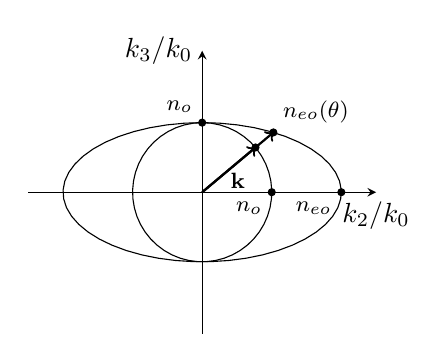
\begin{tikzpicture}


    %\useasboundingbox (-2.5,-1.5) rectangle (3,2.3);
    %\draw (-2.5,-1.5) rectangle (3,2.3);
 
   % 0 \le \left( 1 + \frac{d}{R_1} \right) \left( 1 + \frac{d}{R_2} \right) \le 1
    \begin{axis}[
        axis equal,
        xmin=-2.5,xmax=2.5,
        ymin=-1.5,ymax=1.5,
        axis lines=middle,
        width=60mm,
        xlabel = $k_2 / k_0$, 
        ylabel = $k_3 / k_0$, 
        x label style={anchor=north},
        y label style={anchor=east},
        ticks=none,
        ]
    

        \addplot [domain=0:360, samples=50, black] ({sin(x)}, {cos(x)});
        \addplot [domain=0:360, samples=50, black] ({2*sin(x)}, {cos(x)});

        \draw [->, thick] (0,0) -- (40:1);
        \draw [->, thick] (0,0) -- node[below] {\footnotesize $\mathbf{k}$} (40: {1/sqrt( cos(50)^2 + sin(50)^2 / 2^2)} );
  
       \draw[fill=black] (40:1) circle (0.05) ; %node[anchor= east] {\footnotesize $n_o$};
       \draw[fill=black] (40: {1/sqrt( cos(50)^2 + sin(50)^2 / 2^2)} ) circle (0.05) node[anchor=south west] {\footnotesize $n_{eo}(\theta)$};



        \draw[fill=black] (1,0) circle (0.05) node[anchor=north east] {\footnotesize $n_o$};
        \draw[fill=black] (0,1) circle (0.05) node[anchor=south east] {\footnotesize $n_o$};
        \draw[fill=black] (2,0) circle (0.05) node[anchor=north east] {\footnotesize $n_{eo}$};
    \end{axis}

\end{tikzpicture}


%\end{document}